\documentclass[twoside, 12pt, a4paper]{refart}
\usepackage[utf8]{inputenc}
\usepackage[english]{babel}
% \usepackage[T2A]{fontenc}
\usepackage{amsmath, amsfonts, amssymb, graphicx}
% \usepackage{pscyr}
\usepackage{makeidx}
\usepackage{ifthen}
\usepackage{hyperref}
\hypersetup{colorlinks=true,linkcolor=blue,filecolor=magenta,urlcolor=blue}
\urlstyle{same}

\RequirePackage{caption}
\DeclareCaptionLabelSeparator{defffis}{ -- }
\captionsetup{justification=centering,labelsep=defffis}

\def\bs{\char'134 } % backslash in \tt font.
\newcommand{\ie}{i.\,e.,}
\newcommand{\eg}{e.\,g..}
\DeclareRobustCommand\cs[1]{\texttt{\char`\\#1}}

\title{Microfluidic pressure controller}
\author{
Authors of the manual: \\
% Букатин Антон Сергеевич \\
Ivan A. Denisov \\
% Лукьяненко Кирилл Андреевич \\
% Сорокин Владимир Викторович \\
% Якимов Антон Сергеевич \\
Nikita A. Filatov \\
}



\date{4 Jan 2022}
\emergencystretch1em  %

\pagestyle{myfootings}
\markboth{Manual: Microfluidic pressure controller}%
         {Manual: Microfluidic pressure controller}

\makeindex 

\setcounter{tocdepth}{2}

\begin{document}

\maketitle

\begin{abstract}
The manual includes instructions to assemble, setup and develop open-source microfluidic pressure controller.
\end{abstract}

\tableofcontents

\newpage


%%%%%%%%%%%%%%%%%%%%%%%%%%%%%%%%%%%%%%%%%%%%%%%%%%%%%%%%%%%%%%%%%%%%

\section{Introduction}
\label{intro}

Controller has functions:
\begin{enumerate}

\item control pressure
    
\item control vacuum pump

\item control 8 relays

\item ...
        
\end{enumerate}

\begin{figure}[h!b]
	\begin{center}
	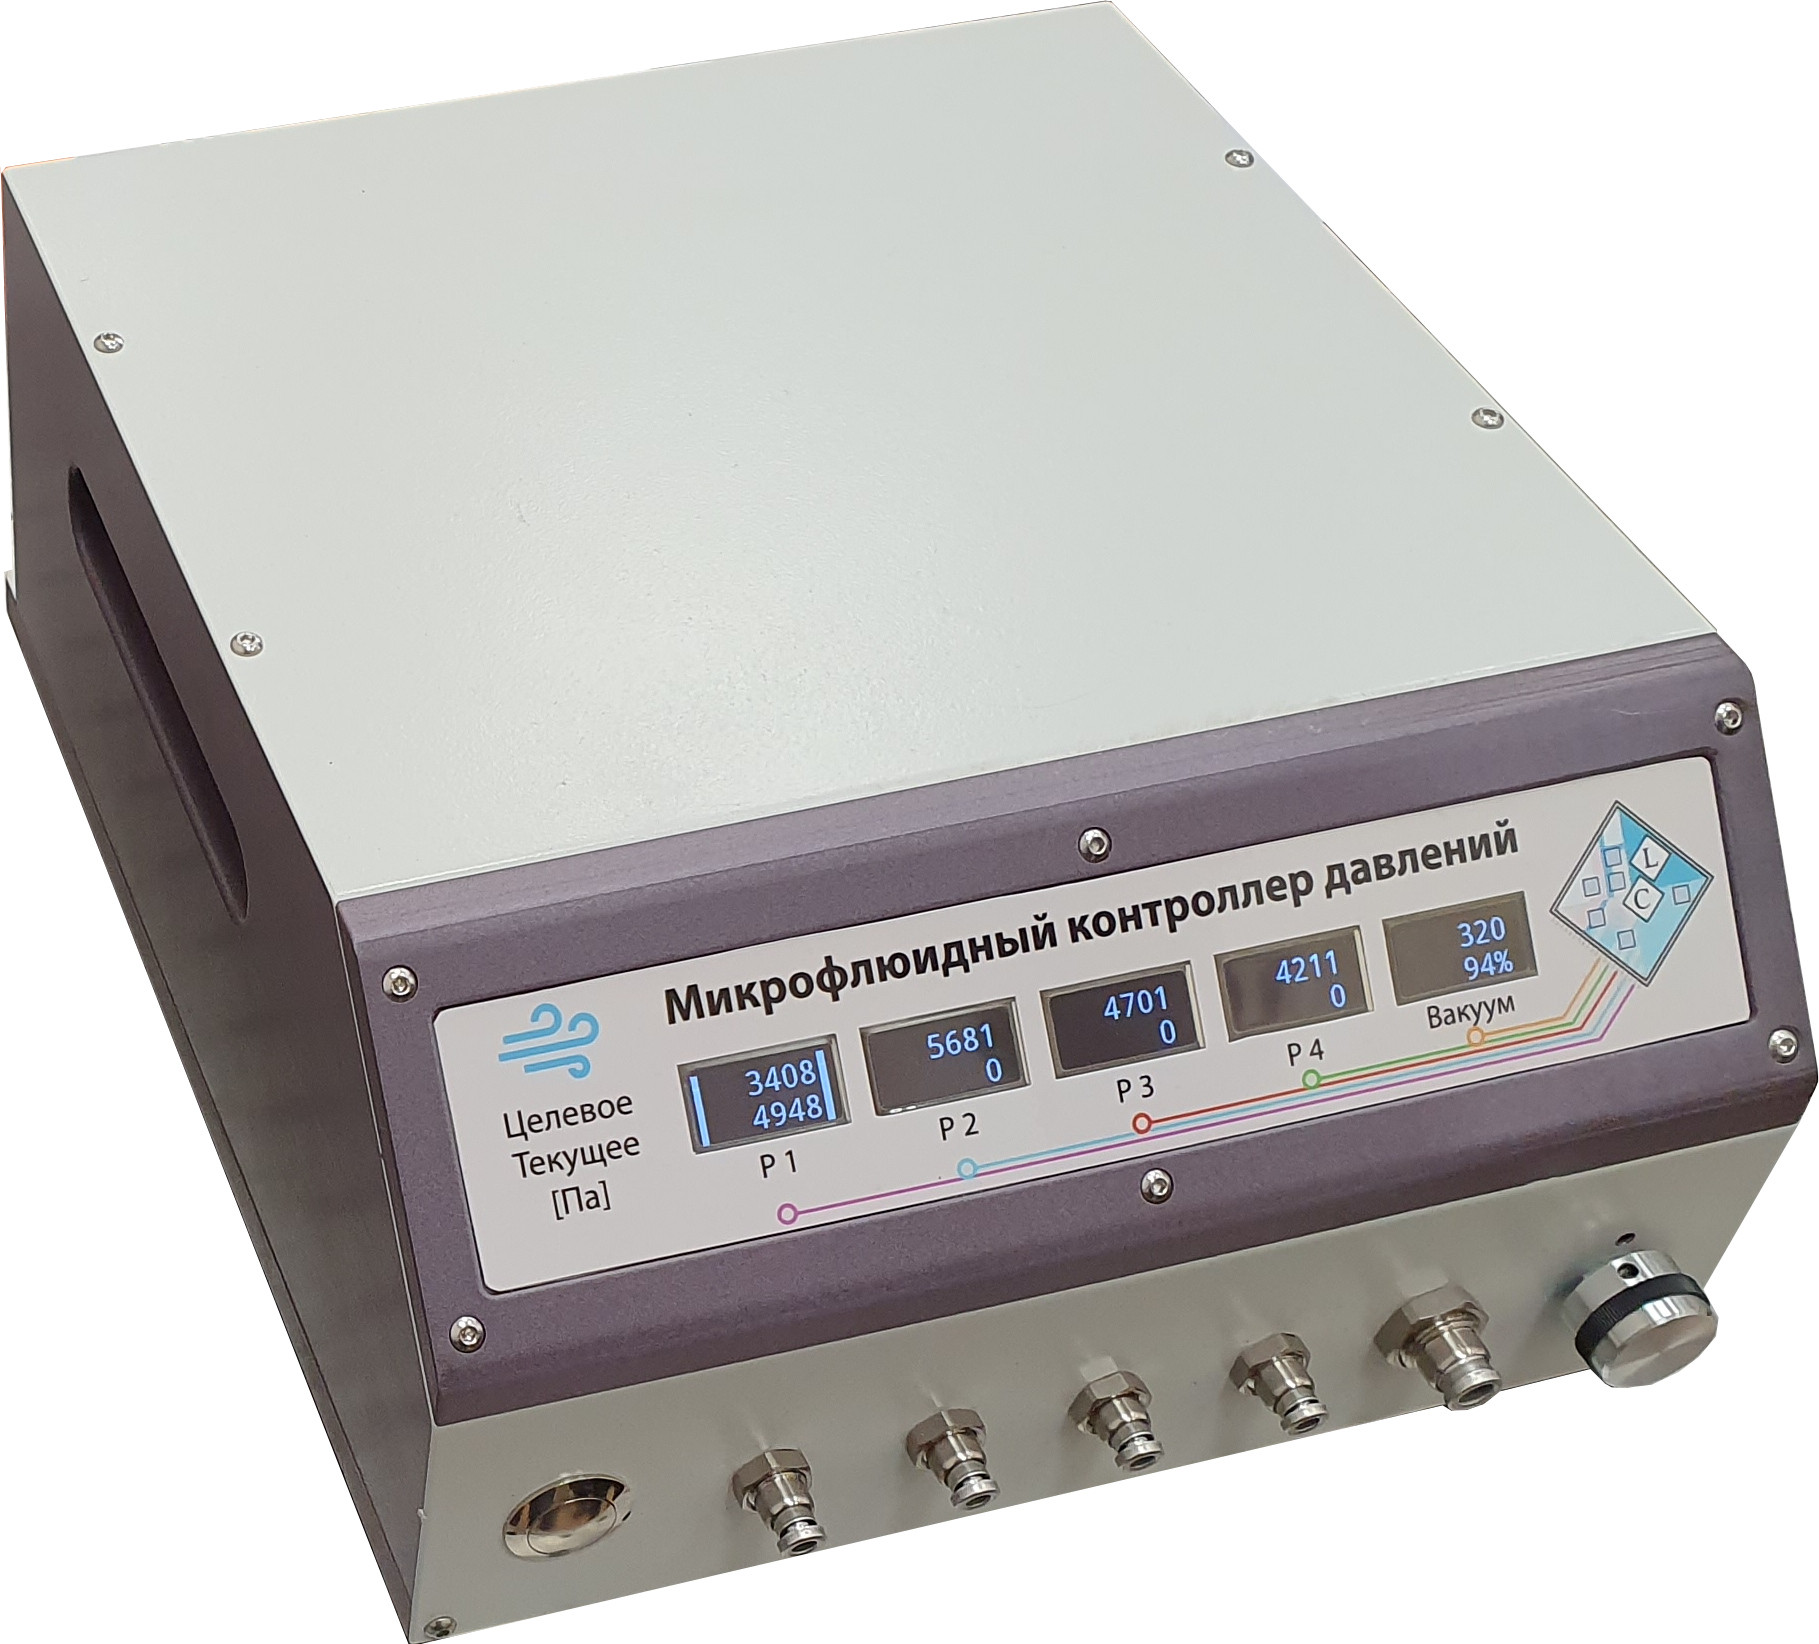
\includegraphics[width=\textwidth]{imgs/device.jpg}
	\caption{exterier}
	\label{fig:device}
	\end{center}
\end{figure}


\subsection{Transportation}

To be written

\subsection{Storage}

To be written

\newpage
\section{Setting up}
\label{setup}


\subsection{Calibration}
 
\begin{description}

\item[Panel for calibration]
%         откройте приложение \textbf{Ветерок}, вызовите справку и найдите кнопку <<калибровка>>.
        
\item[Detectors paramiters]
%         коэффициенты A и B ... 
        

\end{description}

%%%%%%%%%%%%%%%%%%%%%%%%%%%%%%%%%%%%%%%%%%%%%%%%%%%%%%%%%%%%%%%%%%%%%%

\newpage
\section{Usage manual}
\label{usage}

Device can be controlled with physical panel on the front part of the device box or with application with PC.

\subsection{Control panel}

\marginlabel{Encoder:} Device has encoder to change settings ...

\marginlabel{Displays:} Displays informing about  ...


\subsection{Application}




%\attention
%внимание, если задать такую мощность, которая приведет к остановке насоса, то он может перегреться и выйти из строя. Прибор оснащен защитой от пожара (термопредохранитель прикреплен на двигатель насоса), однако срабатывание системы необратимо без ремонта прибора (замены термопредохранителя).



%%%%%%%%%%%%%%%%%%%%%%%%%%%%%%%%%%%%%%%%%%%%%%%%%%%%%%%%%%%%%%%%%%%%%%
\newpage
\section{Developing application}


\printindex

\end{document}
